{

Hvad er et topografisk kort? Eksempler på topografiske kort kan ses i
figur \ref{topography_plus} og \ref{topography_times}.

Vi vil nu beskrive en metode hvorved regioner bliver tildelt en
omkostning. Denne omkostning beregnes ud fra regionens placering i
billedet på baggrund af et topografisk kort. Således vil regioner ikke
blive vurderet efter hvorvidt de ligger i det gyldne snit eller ej, men
efter \emph{hvor meget} de ligger i det gyldne snit.

\subsubsection*{Generation af topografisk kort}

Givet en afbildning af et maleri ved matricen $\mathbf{I}$ med dimensioner
$N \times{} M$, kan man opstille et topografisk kort $\mathbf{T}$ med dimensioner
$N \times{} M$.

Det topografiske kort generes ud fra to vektorer $\mathbf{X}$ og
$\mathbf{Y}$ med dimensioner på henholdsvis $N \times 1$ og $1 \times M$.
\begin{equation}
    \mathbf{X} = \left(
    \begin{array}{c}
        x_1     \\
        x_2     \\
        \vdots  \\
        x_n
    \end{array} \right)
    \label{x_vector}
\end{equation}
og
\begin{equation}
    \mathbf{Y}^{t} = \left(
    \begin{array}{c}
        y_1     \\
        y_2     \\
        \vdots  \\
        y_m
    \end{array} \right)
\end{equation}

Vi betragter vektoren $\mathbf{X}$ som liniestykket givet ved $AB$ i
figur \ref{topograph_line}. Længden af liniestykket betegnes ved $|AB|$.
Det følger af ligning \ref{x_vector} at $|AB| = n$. På liniestykket $AB$
er det gyldne snit placeret ved $G$ hvilket betegner indeks $\lfloor
n\varPhi \rfloor$ i $\mathbf{X}$. Et margin er angivet ved punkterne $(G
- \delta) = m$ og $(G + \delta) = m'$, hvor $\delta$ er størrelsen på
margin. Ligeledes betegner $m$ og $m'$ indeks $\lfloor n \varPhi \pm
\delta \rfloor$ i $\mathbf{X}$.  Endvidere har vi at $|Ap| = \lfloor
\frac{1}{2}|AB| \rfloor \leq |pB|$ og $|m'q| = \lfloor \frac{1}{2}|qB|
\rfloor \leq |qB|$. I figur \ref{topograph_line} er kun liniestykket
$pB$ segmenteret, men $Ap$ segmenteres symmetrisk.

Vi placerer nu et nyt punkt $x$ på $pB$. I det et-dimensionelle plan kan
længden $|Gx|$ bruges som mål for hvor tæt $x$ er på det gyldne snit.
Punktet $x$ har dog ingen udstrækning, hvorfor vi ikke blot kan bruge
længden i praksis. Vi betragter nu en region $R \in \mathbb{Z}^{+}$.
Regionen $R$ er en liniestykke i det et-dimensionelle plan. Vi kan da
udregne placeringen af $R$ i forhold til punktet $G$ ved at summere alle
afstandene fra punkterne $x$ i $R$ til $G$.  Dette medfører at lange
liniestykker bliver tildelt højere værdi end små. Vi udregner således
$\frac{\sum_{x \in R}{|Gx|}}{|R|} = |G(\frac{|R|}{2})|$, hvor $|R|$ er
længden, dvs. antallet af punkter i $R$. Dette svarer til at beregne
afstanden fra regionen midtpunkt til $G$. Dette er ikke ønskværdigt, da
vi kan have to regioner med forskellig længde, men med samme midtpunkt.
Hvis vi lader $R_{max}$ betegne den større region og $R_{min}$ være den
mindre, hvor $ \frac{|R_{max}|}{2} = \frac{|R_{min}|}{2}$, da må
$R_{max}$ nødvendigvis have et ekstrema tættere på $G$ end $R_{min}$.
Det er derfor ikke retfærdigt at give begge regioner den samme værdi.

Vi ønsker at belønne punkter der ligger i eller tæt ved det gyldne snit,
men også omvendt give stor omkostning til punkter der ikke ligger i det
gyldne snit. Til dette bruges vektoren $\mathbf{X}$ som vil angive
omkostningen for hvert punkt på $AB$. Da vi ønsker at belønne punkter i
det gyldne snit er der ingen omkostning til punkter der ligger
i det gyldne snit. Vi sætter derfor $\mathbf{X}_{|AG|}$ til $0$.

\begin{figure}[!h]
    \centering
    \begin{picture}(240,30)
        \put(0, 10){$A$}
        \put(3, -5){\line(0, 1){10}}

        \put(116, 10){$p$}
        \put(118, -5){\line(0, 1){10}}

        \put(131, 10){$m$}
        \put(134, -4){\line(0, 1){8}}

        \put(144, 10){$G$}
        \put(147, -4){\line(0, 1){8}}

        \put(157, 10){$m'$}
        \put(160, -4){\line(0, 1){8}}

        \put(195, 10){$q$}
        \put(198, -4){\line(0, 1){8}}

        \put(233, 10){$B$}
        \put(236, -5){\line(0, 1){10}}

        \put(182, 10){$x$}
        \put(185, 0){\circle*{3}}

        \put(3, 0){\line(1, 0){233}}
    \end{picture}
    \caption[]{Liniestykke}
    \label{topograph_line}
\end{figure}

%Vektorerne angiver omkostningen for at have et punkt i den givne
%dimension. Hvis vi betragter det gyldne snit vil vi gerne have at
%værdierne i $\mathbf{X}_{\lfloor n \varPhi \rfloor}$ og
%$\mathbf{X}_{\lfloor n(1 - \varPhi) \rfloor}$ sættes til $0$, da det
%ikke skal have nogen omkostning at have et punkt i det gyldne snit.
%Ligeledes sættes $\mathbf{Y}_{\lfloor m \varPhi \rfloor}$ og
%$\mathbf{Y}_{\lfloor m(1 - \varPhi) \rfloor}$ også til $0$. Vi bruger
%også her et margin $\sigma$ hvor omkostningen for punkter er lav. Indeks
%$\lfloor n \varPhi \pm \sigma \rfloor$ sættes da til at have
%omkostningen $1$. Dette gøres helt analogt for indeks $\lfloor n(1 -
%\varPhi) \rfloor$ og for vektoren $\mathbf{Y}$.

\begin{figure}[h]
    \setlength\fboxsep{0pt}
    \setlength\fboxrule{0.5pt}
    \begin{center}
        \fbox{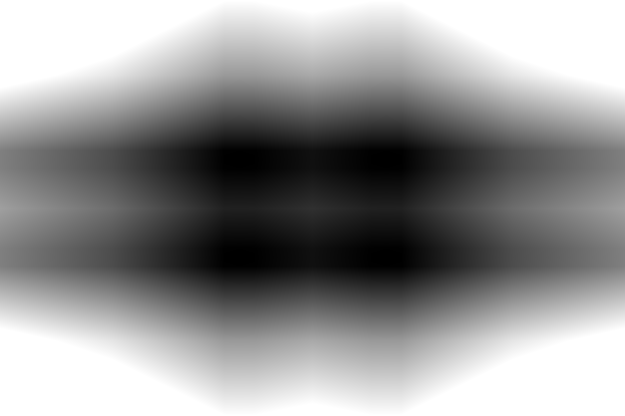
\includegraphics[width=0.8\textwidth]{afsnit/vores_implementation/billeder/udvidet_loesning/topographic_plus.png}}
    \end{center}
    \caption[]{Topografisk kort over omkostninger for regioner ud fra det
    gyldne snit. Værdien $T_{(x, y)}$ er givet ved funktionen
    $t(i, j) = C^{x}_{i} + C^{y}_{j}$ hvor $C^{x}$ og $C^{y}$ angiver
    omkostningsvektorerne.}
    \label{topography_plus}
\end{figure}

\begin{figure}[h]
    \setlength\fboxsep{0pt}
    \setlength\fboxrule{0.5pt}
    \begin{center}
        \fbox{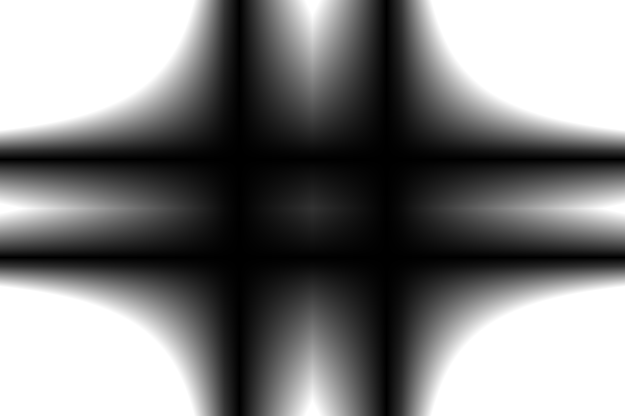
\includegraphics[width=0.8\textwidth]{afsnit/vores_implementation/billeder/udvidet_loesning/topographic_times.png}}
    \end{center}
    \caption[]{Topografisk kort over omkostninger for regioner ud fra det
    gyldne snit. Her er værdierne udregnet ved at multiplicere værdierne
    fra omkostningsvektorene.}
    \label{topography_times}
\end{figure}

\subsubsection*{Omkostningsfunktionen}

Givet en mængde $R \in \{\mathbb{Z}^{+}\times\mathbb{Z}^{+}\}$, som
angiver punkterne i en given region, kan man finde omkostningen
$C$ ved
\begin{equation}
    C(R) = \sum_{(i, j) \in R}{\frac{T_{ij}}{nm}}
\end{equation}

}

% vim: set tw=72 spell spelllang=da:
